\chapter{Background} \label{ch:background}
\section{Machine Learning}
The human beings learn by experience, part of which is inherited from previous generations. In the digital world, the experience can be represented in form of data, which can be later processed and analysed.

We live in the data deluge era. The technological progress and the internet have boosted our logging and communication capacities. At the time of writing this paragraph\footnote{https://www.internetlivestats.com/one-second/ on February 6th 2022}, every single second one second 10,000 new tweets are written, 100,000 searches are sent to \textit{Google}, 100,000 videos are viewed in \textit{YouTube}, and 3,000,000 emails are sent. All amounts to approximately a 140 TB of internet traffic per second. 

This Brobdingnagian amount of data cannot be analysed without the help of automated computational assisted tools, and this is exactly the purpose of machine learning. More formally, we define machine learning as a set of computational methods designed to automatically learn hidden structures and patterns from the data and its origin \cite{murphy2012, theodoridis2015}. Machine learning algorithms can serve multiple purposes ranging from informing decision making under uncertainty to understand and simulate natural processes.

Sometimes, machine learning algorithms are inspired in biological processes or in how the brain works and learns \cite{haykin1998} (e.g. self-organising maps \cite{kohonen2001}). Other times, machine learning is driven by specific needs arising from data analysis problems (e.g. binary decision trees \cite{hastie2009, hastie2014}).

\section{Types of learning}
One commonality of all Machine learning algorithms is that they are designed to learn from data. However, there are many ways these data can be treated in the learning process. In this section, the most common types of learning are described.

\subsection{Supervised learning}
Supervised learning is the most widely employed methodology to train machine learning models. It is based on a function-fitting perspective, where the function is adjusted (or trained, in machine learning terms) to map a set of input vectors $\mathbf{X}$ to the corresponding output vectors $\mathbf{Y}$ ($f_\theta:\mathbf{X}\rightarrow \mathbf{Y}$), given a labeled set of $N$ input pairs $\mathbf{T}=\{(\mathbf{x_i},\mathbf{y_i})\}_{i=0}^{N}$ known as the training set \cite{theodoridis2015}. The learning algorithm changes the parameters $\theta$ of the function $f$ according to the minimization of a predefined cost function $J$ (for example the mean squared error between the predicted values and the labels) \cite{hastie2009}. The vector $\mathbf{x_i}$ (with length $D$) represents a set of features (for example the age and the income of a person)  and $\mathbf{y_i}$ (with length $K$) is the a vector of response variables (representing for example the credit score and the propensity to buy a certain product)\footnote{Notice that we denote $\mathbf{y_i}$ as a vector although supervised models can be univariate. However the multivariate form is a more general case.}.

There are two main forms of supervised learning  \cite{murphy2012}.

\begin{itemize}
	\item Regression, where the task consists of mapping each input vectors $\mathbf{x_i}$ to a real-valued vector $\mathbf{y_i} \in \mathbb{R}^K$. An example of this task would be predicting the age of an abalone\footnote{a type of marine snail} based on physical measurements of the different parts of its body \cite{dua2019abalone}.
	\item Classification, where a task consists of mapping the input vectors $\mathbf{x_i}$ to nominal variables from a finite set $y_{i,j} \in {1,2,...,C_j}$, where $C_j$ is the cardinality of the $j$-th output set. An example of a classification task would be determining if a mushroom is poisonous or edible based of several physical characteristics \cite{dua2019mushroom}.
\end{itemize}

\subsection{Unsupervised learning}
Unsupervised learning techniques are employed when no labeled data is available. The training data set is composed of only input vectors $\mathbf{T}=\{(\mathbf{x_i})\}_{i=0}^{N}$, and the objective consists of finding interesting patterns in the data. Unsupervised learning comprises a wider range of techniques, as compared to supervised learning, and its objective is less well defined because the models have no clear desired output nor obvious error metric. However, the unsupervised learning paradigm to be closer to how animals and humans learn. These algorithms also provide a cheaper framework for data exploitation, given that no data annotation is required by human experts, which is generally expensive. 

Some of the most common forms of unsupervised learning are described below.

\begin{itemize}
	\item Clustering: consists of finding dissimilar subpopulations in the data (also known as clusters or groups), where the elements of a sub-population are more similar to each other than to elements in other sub-populations.
	\item Density or probability mass estimation: the machine learning algorithm is trained to learn the probability density function of the data (or the probability mass function in case $X$ is discrete) $p_{model}(\textbf{X}): \mathbb{R}^N \rightarrow \mathbb{R}$ \cite{Goodfellow2016}. For this, the model needs to learn the underlying structure of the data $\mathbf{X}$. The techniques laying in this family can be used for many downstream applications, such as clustering \cite{wang2006}, missing data imputation \cite{qichuan2015} or generation \cite{liu2020}. 
	\item Manifold learning: is set of techniques consisting of learning the structure of high-dimensional data, where the data is assumed to lie on a low-dimensional manifold in a high-dimensional space. The objective of these techniques is to discover latent structures in the data that can be exploited for tasks such as data compression, dimensionality reduction, feature extraction or data visualization. One example of this task would be reducing the dimensionality of a data set using Principal Component Analysis (PCA), which would project the original data set into a lower-dimensional one with ortogonal axes, where the structures in the data would be more easily discernible.
	\item Data completion: consists of imputing the missing values of a given data set \cite{vanburen_2018}. This can be done with different purposes such as inferring the unfilled optional answers of a survey, or filling the gaps of a time series with low sampling frequency to get a higher time resolution representation. Some forms of collaborative filtering \cite{falk2019}, for example matrix factorization algorithms \cite{koren2009}, can also be seen as a data completion task where the algorithm needs to fill the blanks of a matrix representing the ratings of products by customers.
	\item Associative learning:  is a type of unsupervised learning where the goal is to discover the relationships between objects in the data \cite{zhang2002}. These relationships can be expressed in terms of associations (e.g. if A then B), correlations (e.g. A is positively correlated with B) or co-occurrence (e.g. A and B are often observed together). One example of associative learning would be applying the \textit{Apriori} algorithm \cite{agrawal1996} to a supermarket database in order to discover the most interesting associations between different products with the aim of deriving attractive offers for customers. 
	\item Generative modeling: many forms of generative model also rely on unsupervised learning techniques \cite{bishop2006}. This task consists of learning to approximate $P(\mathbf{X})$ with the objective of generating data that is indistinguishable from the original distribution, and it is done usually by maximizing the likelihood of the data given the model $\mathrm{argmax}_\mathbf{\theta} P(\mathbf{\mathbf{X},\mathbf{\theta}})$.  One example of application of these techniques would be in the field of natural language processing, where the goal is to learn a model that can generate text \cite{uday2019} that is realistic and linguistically plausible (these are known as language models). 
\end{itemize}


\subsection{Reinforcement Learning}
Reinforcement learning is a family of machine learning algorithms which, in contrast to the other types of learning, does not necessarily rely on any previous knowledge about the task at hand. Instead, the reinforcement learning agents (or decision makers) learn what to do by mapping situations to actions \cite{sutton2018} so that they maximize a numerical reward signal, usually in presence of uncertainty \cite{haykin1998}. For the agent to learn successful behaviors (referred commonly as policies), they need to balance exploration and exploitation while interacting with the environment \cite{sutton2018}, in other words, reinforcement learning algorithms learn by trial and error. 

More formally, the environment is commonly formulated as \textit{finite-discrete-time Markov Decision Process} \cite{haykin1998}, which can be represented as a 4-tuple: ($S$, $A$, $P_a$, $R_a$) where $S$ represents the state space, $A$ is the action space, $P_a(s, s')$ is the probability of transitioning from state $s$ to state $s'$ after choosing the action $a$, and $R_a(s, s')$ is the reward received at transitioning from state $s$ to state $s'$ after performing action $a$. The objective of the learning algorithm is to build an agent such that its policy $\pi_\theta(s)$ maximizes the expected sum of discounted rewards $\mathbb{E} \left[ \sum_{t=0}^{T} \gamma^t R_a(s_t, s_t+1) \right]$, where $\gamma$ is usually a scalar number between 0 and 1 that is exponentially decayed to 0 as time $t$ increases. The reinforcement learning theory is originally based upon dynamic programming \cite{szepesvari2010}. 

A classical example commonly found in the literature of a successful reinforcement learning application can be found in \cite{tesauro1994}, where a reinforcement learning algorithm is trained to play \textit{Backgammon} game.

Detail treatment of the reinforcement learning field lies far beyond the scope of this thesis. A more detailed introduction is given in the following references: \cite{sutton2018, szepesvari2010}.

\subsection{Other types of learning}
There are other types of learning \cite{raghu2020} that are worth mentioning but either it is not clear where they lay, or they combine elements from the previously discussed types of learning. The following list describes the most important ones.
\begin{itemize}
	\item Semi-supervised learning algorithms learn from both labeled and unlabeled data. This is beneficial in problems where it is difficult or costly to label the data, and the amount of labeled data is scarce \cite{raghu2020}. One example of field where semi-supervised learning applications apply is fraud detection \cite{wang2020}.
	\item Self-supervised learning algorithms aim to solve what is known a \textit{pretext task}: a supervised problem where the data can be automatically labeled without human intervention, without extra cost and directly from the raw instances \cite{raghu2020}. One example of \textit{pretext task} could be determining the missing word in a masked sequence, given a set of sentences extracted from a collection of books \cite{devlin2019}, or determining the degree of rotation of an image \cite{gidaris2018}.
	\item Transfer learning is solely applicable to deep learning models. This methodology consists of two steps: pre-training a model to solve a large and generic task (e.g. classify large and full-color images into 1000 categories \cite{deng2009imagenet}) and then fine-tune the pre-trained model to solve a target task \cite{raghu2020}. This paradigm has a lot of benefits in multiple applications (for instance when small amounts of labeled data are available, or when the computational resources available are limited). As an example, \textit{Souza and Filho} \cite{souza2022} show how they got successful results in performing sentiment analysis over user reviews by using pre-trained word embeddings based on \textit{BERT} (\cite{devlin2019}). Further details about transfer learning will be covered in this thesis in a following chapter.
\end{itemize}


\section{Deep Learning}

Deep learning algorithms were motivated by the failure of classical machine learning algorithms on solving central problems on AI (e.g. speech recognition, object recognition, text generation, etc). These algorithms have a long history (figure \ref{fig:dl-timeline} summarizes the most important events in the development process of these algorithms), and have been named differently along the years: connectionist models, artificial neural networks, etc.  

\begin{figure}
	\centering
	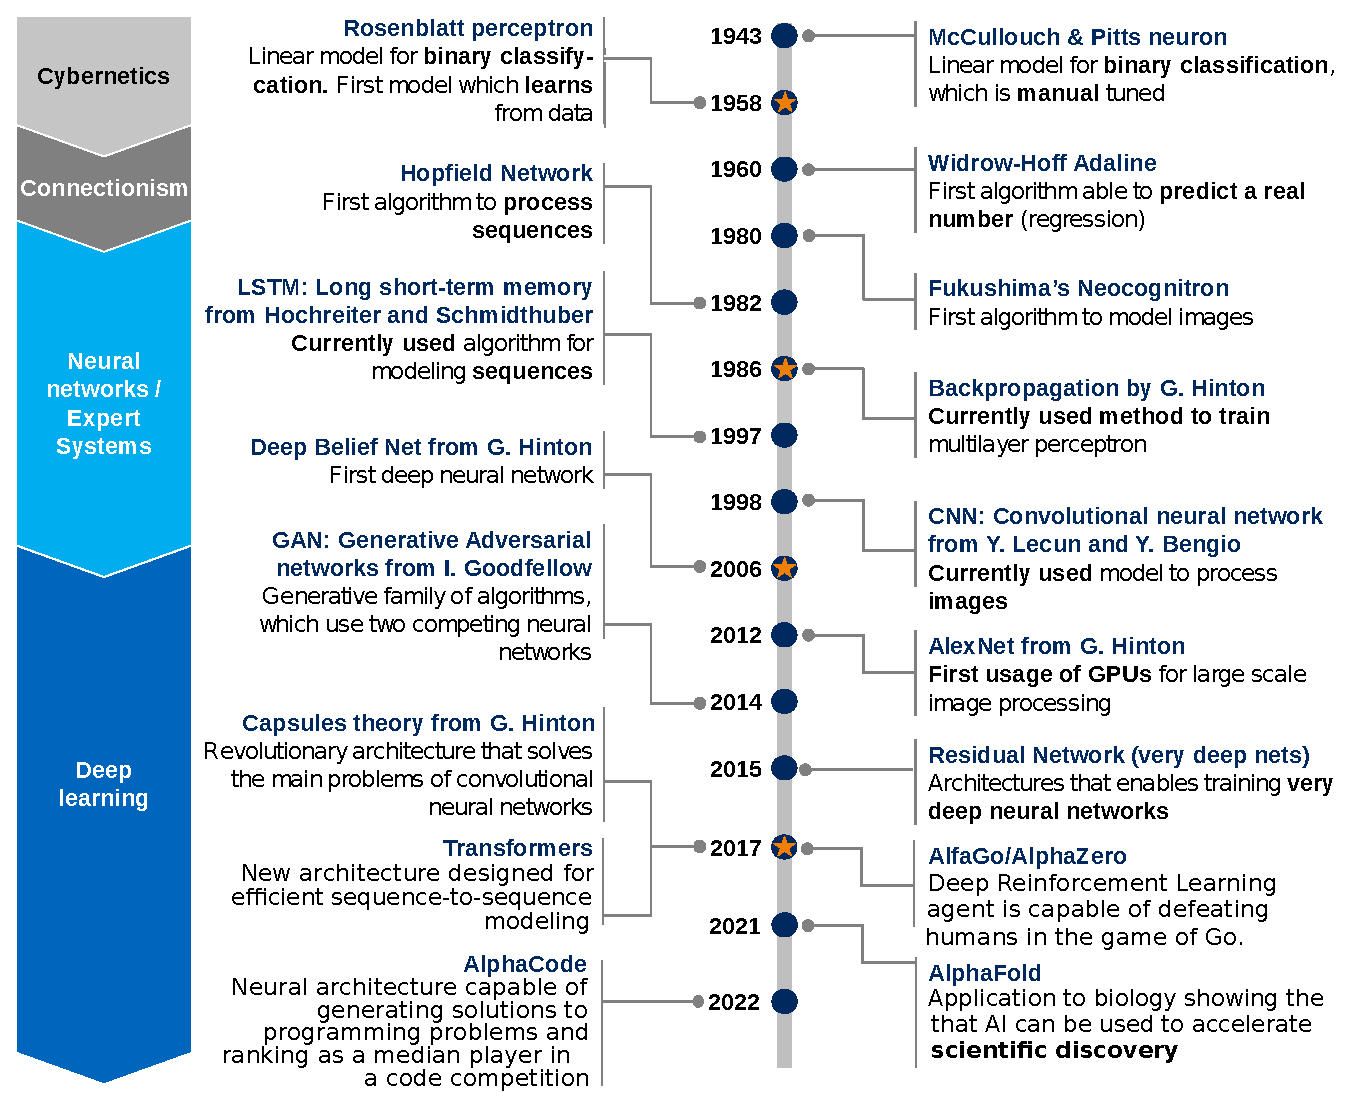
\includegraphics[width=1.0\linewidth]{chapter2/images/DL-timeline}
	\caption{Timeline showing the most important achievements in the research of what is currently known as deep learning algorithms.}
	\label{fig:dl-timeline}
\end{figure}


Deep Learning is a subfield of artificial intelligence and machine learning as shown in the \textit{Venn} diagram of figure \ref{fig:venndl} (taken from \cite{Goodfellow2016}), and provides a very flexible framework for different machine learning tasks spanning all the aforementioned types: supervised, unsupervised, reinforcement learning and others.

\begin{figure}
	\centering
	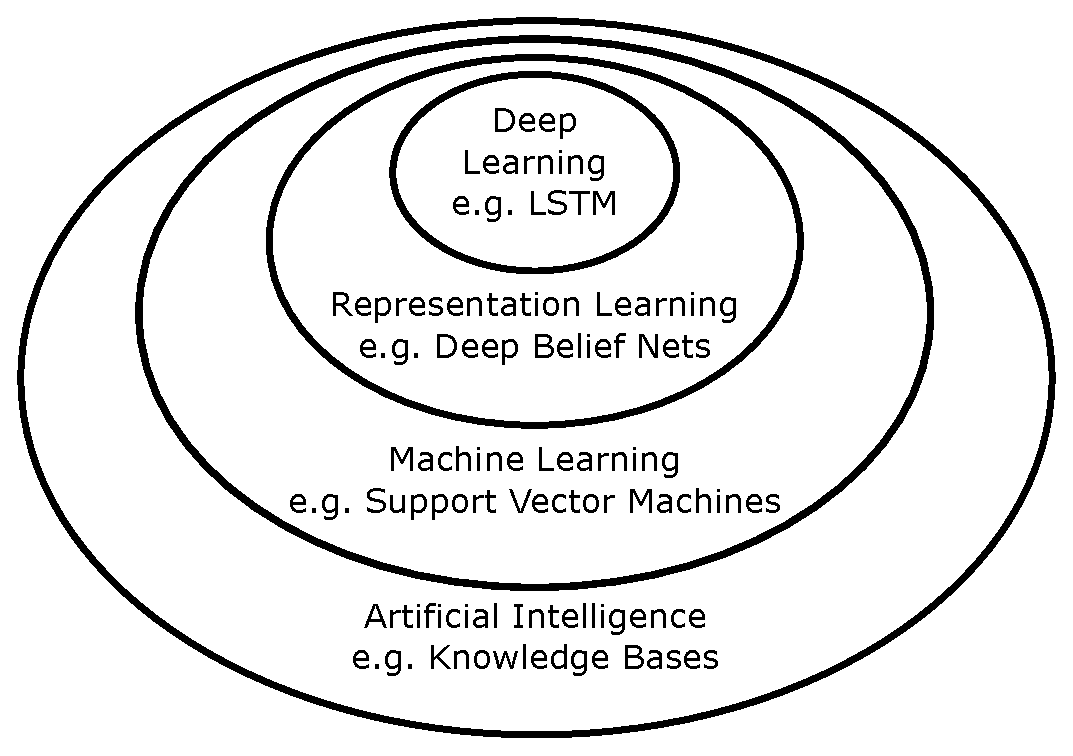
\includegraphics[width=0.5\linewidth]{chapter2/images/venn_DL}
	\caption{Deep learning context within the artificial intelligence field \cite{Goodfellow2016}}
	\label{fig:venndl}
\end{figure}



\subsection{From the perceptron to its multilayer version}

This section introduces the basic feed-forward neural network, from its origin to the modern trends. The basic component of a modern deep learning model is the neuron (sometimes called unit). The idea of neuron has its origin in the \textit{McCulloch and Pitts} model from 1943, an attempt to mathematically model the functionality of a biological network \cite{mccullochPitts1943}. The \textit{McCulloch and Pitts} model consisted on a linear function of a set of binary inputs $\mathbf{x}$ that is multiplied by a set of weights $\mathbf{W}$ (which value is either excitatory or inhibitory, i.e. 1 or -1), the result is added together and a sign function is applied to produce a binary output $y$ (see figure \ref{fig:mcpittsneuron} for a graphical description). The whole model is described in equation \ref{eq:mcpitts} This algorithm was meant to be adjusted manually by an operator.

\begin{figure}
	\centering
	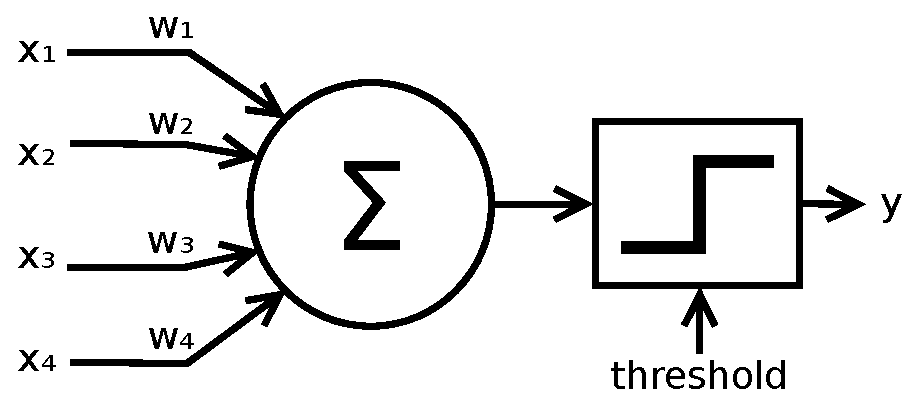
\includegraphics[width=0.4\linewidth]{chapter2/images/mcpittsneuron}
	\caption{McCulloch and Pitts model, with 4 input variables $\{x_i\}$ and one output $y$.}
	\label{fig:mcpittsneuron}
\end{figure}

\begin{equation}
	\label{eq:mcpitts}
	y_i = \mathrm{sgn}\left(\sum_{j=0}^{D} x_{i,j} \cdot w_{j} \right) 
\end{equation}

Some years later (1958), \textit{Frank Rosenblatt} introduced the \textit{Perceptron} \cite{Rosenblatt58}. His idea builds upon the \textit{McCulloch and Pitts} model, proposing a \\
ple method to automatically learn the weights of the model (equation \ref{eq:rosenblatt}). This is considered the first primitive neural network.

\begin{equation}
\label{eq:rosenblatt}
\mathbf{w_j(t+1)} = \mathbf{w_j(t)} + (y_j-\hat{y}_j(t))\cdot \mathbf{x_j}
\end{equation}

 A couple of years later, \textit{Bernard Widrow} and his student \textit{Ted Hoff} proposed the \textit{ADALINE} model (ADAptive LINear Element) \cite{widrow1960}, a modification of the \textit{McCulloch and Pitts} model that introduced a bias term and removed the sign function. \textit{ADALINE} was trained using gradient descent, as described in equations \ref{eq:adaline_gd} and \ref{eq:adaline_step}, where $\lambda$ is the learning rate. 
\begin{equation}
\label{eq:adaline_fp}
y_i = \sum_{j=0}^{D} x_{i,j} \cdot w_{j} + b
\end{equation}

\begin{equation}
\label{eq:adaline_gd}
\frac{dJ}{d{w_j}} = \frac{1}{N} \sum_{i=1}^{N} x_{i,j} \cdot(\hat{y}_i - y_i)
\end{equation}

\begin{equation}
\label{eq:adaline_step}
\mathbf{w_j(t+1)} = \mathbf{w_j(t)} - \lambda \cdot \frac{dJ}{d{w_j}}
\end{equation}


 The combination of multiple \textit{ADALINE}-style perceptrons builds a \textit{multilayer perceptron} (\textit{MLP}). More specifically, an \textit{MLP}, also known as \textit{feed-forward} or \textit{fully-connected} neural network, is a neural architecture built with perceptrons (called neurons in this scenario) which are disposed in layers so that all the elements from a layer $l$ are connected with all the elements in the next layer $l+1$ (refer to figure \ref{fig:mlp} as an example)
 
 
 The \textit{ADALINE} training method built the basis for the \textit{backpropagation} algorithm, a widely used methodology nowadays as standard method to train neural networks. The \textit{backpropagation} algorithm \cite{hinton1986} was published by \textit{David Rumelhart} and \textit{Geoffrey Hinton} in 1986 as a method to optimize the parameters of a \textit{multilayer perceptrons}. The algorithm consists of two steps:

\begin{enumerate}
\item Forward pass: consisting of a simple model inference, where a set of features $\mathbf{x}_i$ are feed to the network as input to get the output $\mathbf{\hat{y}_i}$. In this phase, some of the values of the intermediate neurons can be cached to use them in the next step.

\item Backward pass: an error metric is used to compare the outputs of the model $\mathbf{\hat{y}_i}$ with the desired outputs (sometimes called targets) $\mathbf{y}$ and then propagate the gradient of the error backwards (from the output to the input), by using the chain rule, to adjust the weights of the model. 
\end{enumerate}


\begin{figure}
	\centering
	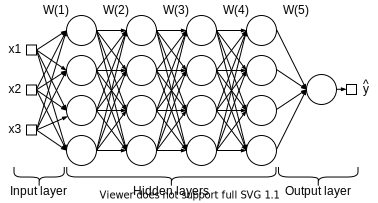
\includegraphics[width=0.5\linewidth]{chapter2/images/mlp}
	\caption{Example of Multilayer Perceptron with 3 inputs, 3 outputs and 3 hidden layers.}
	\label{fig:mlp}
\end{figure}


Before \textit{backpropagation}, there was no algorithm for training \textit{multilayer perceptrons} in an end to end manner. The only way to train those models was to fix the weights of all but one layer, and train the free one with gradient descent. These models were called feature analyzers \cite{hinton1986}, and one of the most important examples is the \textit{Gamba} perceptrons, introduced by described in \cite{minsky69perceptrons}. Although it is out of the scope of this thesis, it may be worth mentioning modern versions of the \textit{Gamba perceptron} (known as \textit{Extreme Learning Machines}) are still in the community research spectrum (see \cite{Huang2006, Huang2012}), as alternative training methods to \textit{backpropagation}.

The introduction of \textit{backpropagation} allows the neural networks to learn their own hidden representations automatically, allowing for more complex and abstract models. One of the most important pieces of \textit{multilayer perceptrons} and other modern architectures are the neuron \textit{activation functions} (also referred sometimes as \textit{nonlinearities}). An \textit{ADALINE} style neuron is a linear function, and linear functions are closed under composition, therefore, the composition of several \textit{ADALINE} neurons is a linear function. To break the linearity of the neurons, the \textit{activation functions} are introduced. They consist of non-linear functions applied to the output of each neuron. The authors of \cite{hinton1986} formulated the \textit{backpropagation} algorithm with sigmoid activation functions (defined in equation \ref{eq:sigmoid}), as a differentiable alternative to the classical sign function. Later, it was discovered that unbounded \textit{nonlinearities} like the \textit{Rectified Linear Unit} (\textit{ReLU}) \cite{nair2010} (defined in equation \ref{eq:relu}), would perform better on training deep architectures. We cover discuss more in depth the activation functions topic in a following chapter. %TODO: Add ref.


\begin{equation}
\label{eq:sigmoid}
f(x) = \frac{1}{1+e^{-x}}
\end{equation}

\begin{equation}
\label{eq:relu}
f(x) = \max(x, 0) =
\begin{cases}
1,          & \text{if } x \geq 0 ,\\
0,         & \text{otherwise},
\end{cases}
\end{equation}

The \textit{backpropagation} algorithm is has certain rules that have to be met \cite{hinton1986}: (1) connections from higher level neurons to lower level ones are forbidden, but connections that skip layers are totally permitted, (2) the architecture must be fully differentiable to be able to back-propagate the errors and (3) the weights must not be initialized to constant values, but they must be set to random values instead, to break the symmetrical weights between layers (which would cause the optimization to stall, see \cite{hinton1986} for more details). Despite meeting these rules, there are no theoretical guarantees for the algorithm to raise the global minimum, it can get stuck in local minima. One possible way to avoid this problem consists of training the model several times with different random initializations \cite{haykin1998}.

\subsection{Neural networks as universal approximators}


\subsection{Deeper neural networks}
Regardless the emergence of the \textit{backpropagation} algorithm, training a \textit{multilayer perceptron} with many layers was \textit{challenging}. The first successful methodology for training deep neural networks consisted on pre-training the weights of the network in an unsupervised fashion, using stacks of \textit{Restricted Boltzmann Machines} (RBM) \cite{Smolensky1986} known as Deep Belief Networks \cite{hinton2006, Bengio2007}. A \textit{Restricted Boltzmann Machine} (initially called \textit{Harmonium}) consists of a type of neural network built using a bidirectional bipartite graph architecture, with symmetric connections of neurons between the two layers and without connections between neurons within the same layer (as shown in figure \ref{fig:rbm}. This model is trained to learn hidden abstract representations of the input, from which it is possible to recover the original probability distribution $P_\theta(x|h) \approx P(x)$. The training procedure is based on an approximate \textit{Maximum-Likelihood} method called \textit{Contrastive Divergence (CD)} \cite{hinton2002}.

\begin{figure}
	\centering
	\includegraphics[width=0.2\linewidth]{chapter2/images/rbm}
	\caption{\textit{Restricted Boltzmann Machine} with 5 visible units and 3 hidden units.}
	\label{fig:rbm}
\end{figure}

Deep Belief Networks are stacks of RBMs that are trained in a greedy layer-wise fashion, in which the output of a trained RBM becomes the input of the following RBM \cite{hinton2006} (see figure \ref{fig:dbn}). It was shown in \cite{Bengio2007} that by following this procedure and then fine-tuning the weights of the full network using the backpropagation algorithm, deeper networks could be trained. 




At the time of writing this thesis, unsupervised pre-training methods are no longer needed to train deep neural networks. This is thanks to a set of techniques that have been recently developed (in the 21st century) and that, when combined together, enable the \textit{backpropagation} algorithm to efficiently optimize deep architectures. The first technique was the usage of ReLU activation functions \cite{nair2010} (eq. \ref{eq:relu}), a non-saturating alternative to the classical functions like \textit{sigmoid} (eq. \ref{eq:sigmoid}) or \textit{tanh}, that showed to be effective at favoring sparse connectivity, and helped overcome the saturating gradients problem, a well known failure mode of neural architectures with saturating \textit{nonlinearities} trained by \textit{backpropagation} \cite{Hong2019}. See figure \ref{fig:relu}. Another technique that helped training deep neural networks is known as \textit{Dropout}, a regularization technique that consists of randomly zeroing out a fraction $p$ of neurons from each layer in each training step \cite{hinton2012, srivastava2014}. These two techniques (among others) allowed \textit{Alex Krizhervsky} and collaborators to successfully train \textit{AlexNet} without unsupervised layer-wise pretraining, a deep neural network that won the \textit{ImageNet} \cite{deng2009imagenet} computer vision contest in 2012, a problem consisting of classifying millions of images into 1,000 categories. These techniques are still used today in the majority of the deep learning models that are published. 

\begin{figure}
	\centering
	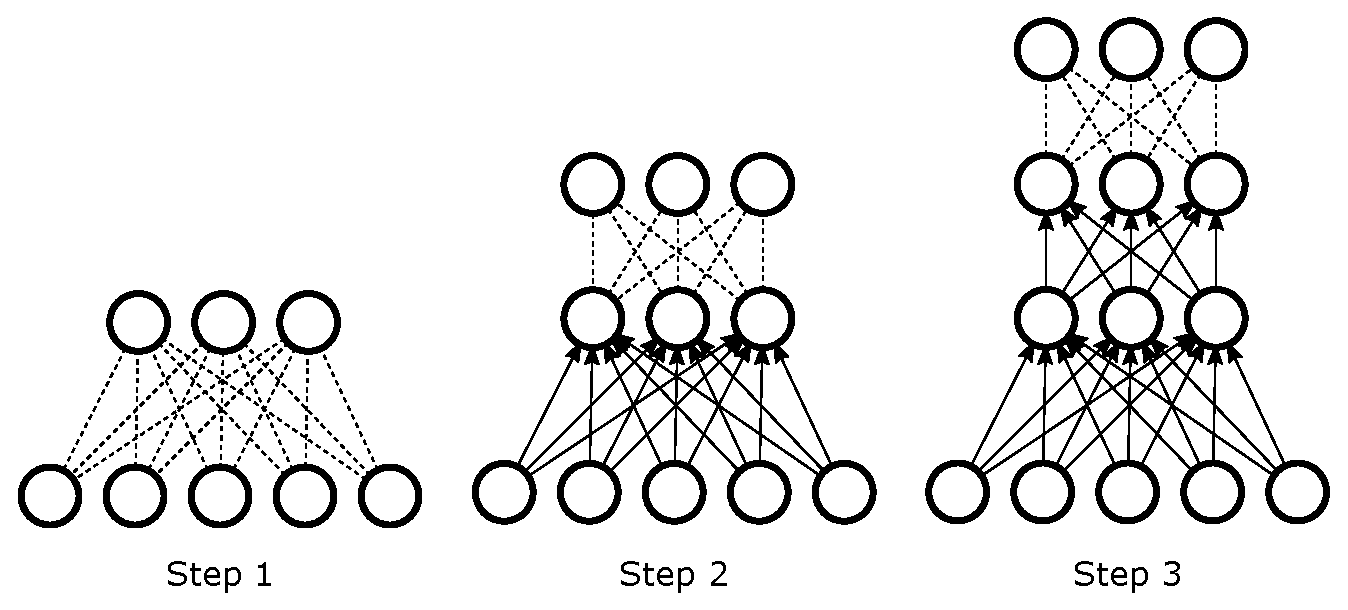
\includegraphics[width=0.7\linewidth]{chapter2/images/dbn}
	\caption{Example of \textit{Deep Belief Network} architecture with three feature detector layers. In each of the steps shown above, the dashed connections between units represent the \textit{RBM} being trained, while the solid connections represent the previously trained \textit{RBMs} that are used to compute the input of the next \textit{RBM}.}
	\label{fig:dbn}
\end{figure}


\begin{figure}
	\centering

		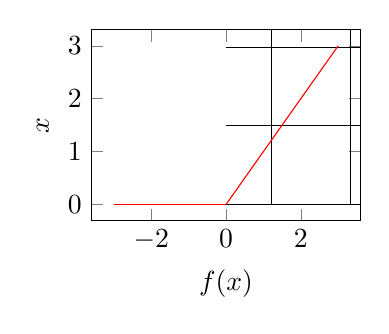
\begin{tikzpicture}
			\begin{axis}[
				domain=-3:3,
				xlabel={$f(x)$},
				ylabel={$x$},
				width=5cm,
				height=4cm,
				]
				\draw[step=1cm,black,very thin] (0,0) grid (5,5);
				\addplot+[mark=none,red,domain=-3:0] {0};
				\addplot+[mark=none,red,domain=0:3] {x};
			\end{axis}
		
		\end{tikzpicture}
	\caption{Rectified linear unit function}
	\label{fig:relu}
\end{figure}

Other tricks that are commonly used nowadays to facilitate the parameters optimization of deep architectures are batch normalization \cite{ioffe2015} and residual learning \cite{kaiming2016}. Batch normalization consists of standardizing the output vectors from hidden layers using the first and the second statistical moments (mean and variance) of the current batch \cite{ioffe2015}. This method has proved to increase the training stability when high learning rates are used \cite{Goodfellow2016}. Additionally, it has been shown that it provides regularization \cite{dauphin2021}, as a side effect, due to the random fluctuations in the statistical moments from one batch to another. Residual learning consists of adding skip connections between layers of the neural network, so that the output of one layer $l$ is fed as input to layer $m > (l+1)$. Figure \ref{fig:residual} shows an example of a graph with a residual block skipping two layers. More formally, the output of the residual block becomes $\mathbf{H(x)} = \mathbf{F(x)} + \mathbf{x}$ where $\mathbf{F(x)}$ is the function learned by the composition of the two layers and the \textit{ReLU} function which, obviously one can see that $F(x)$ is learning a residual mapping $\mathbf{F(x)} = \mathbf{H(x)} - \mathbf{x}$ \cite{kaiming2016}. This method has empirically shown substantial improvements of the \textit{backpropagation} optimization process. The authors of \cite{kaiming2016} were able to get the first place in the \textit{ImageNet} contest in 2015, improving the performance of \textit{AlexNet}. Recent studies found that residual connections help reform the loss landscape leading to more convex optimization surfaces \cite{freeman2017, wang2020}.


\begin{figure}
	\centering
	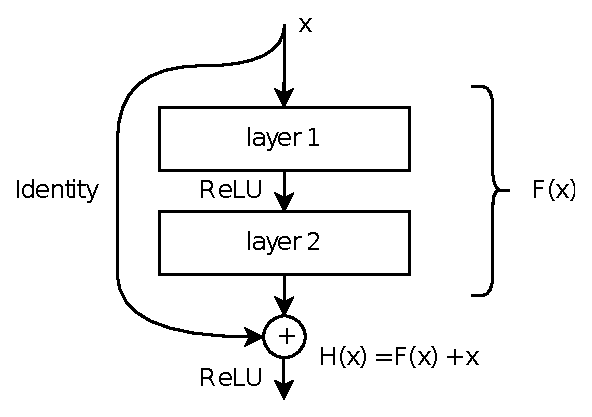
\includegraphics[width=0.5\linewidth]{chapter2/images/residual}
	\caption{Example of a residual block.}
	\label{fig:residual}
\end{figure}


Finally, another difference between modern and classical deep learning models is the extended use of \textit{mini-batch} stochastic gradient descent (see equation \ref{eq:mbsgd}), where successive optimizations steps are performed by \textit{backpropagation} using small ($m$-sized) random sub samples of the dataset named \textit{mini-batches} \cite{ruder2016}. Previous alternatives were stochastic gradient descent, where the updates are performed for every individual sample, and batch gradient descent, where the updates are performed over the full data set $\mathbf{T}$. \textit{Mini-batch} gradient descent has shown generalization improvements over the batch method \cite{Hoffer2017}, while being computationally more efficient than the \textit{stochastic gradient descent} method.
	

\begin{equation}
	\label{eq:bgd}
	\mathbf{\theta(t+1)} = \mathbf{\theta(t)} - \lambda \cdot \mathbf{\nabla_\theta J(X, Y|\theta(t))}
\end{equation}
	
\begin{equation}
	\label{eq:sgd}
	\mathbf{\theta(t+1)} = \mathbf{\theta(t)} - \lambda \cdot \mathbf{\nabla_\theta J(x_i, y_i|\theta(t))} \quad \mathrm \quad \mathrm{where} \quad (\mathbf{x_i}, \mathbf{y_i}) \sim \mathbf{T}
\end{equation}

\begin{equation}
	\label{eq:mbsgd}
	\mathbf{\theta(t+1)} = \mathbf{\theta(t)} - \lambda \cdot \mathbf{\nabla_\theta J(x_{i:i+m}, y_{i:i+m}|\theta(t))} \  \mathrm{where} \quad  (\mathbf{x_{i:i+m}}, \mathbf{y_{i:i+m}}) \sim \mathbf{T}
\end{equation}


\subsection{Modern architectures}
% Transformer, rnn, cnn

\subsection{Generative deep learning models}
% NormFlow, GAN, VAE, AR
